\chapter{System Architecture}
\label{ch:system-architecture}

\section{Overview}

Expo Snips is a two-client, one-engine system. There is no server tier: the only
network-facing component is a set of static JSON documents, and both clients can
operate entirely without it because the catalog is embedded at build time.

\begin{figure}[H]
\centering
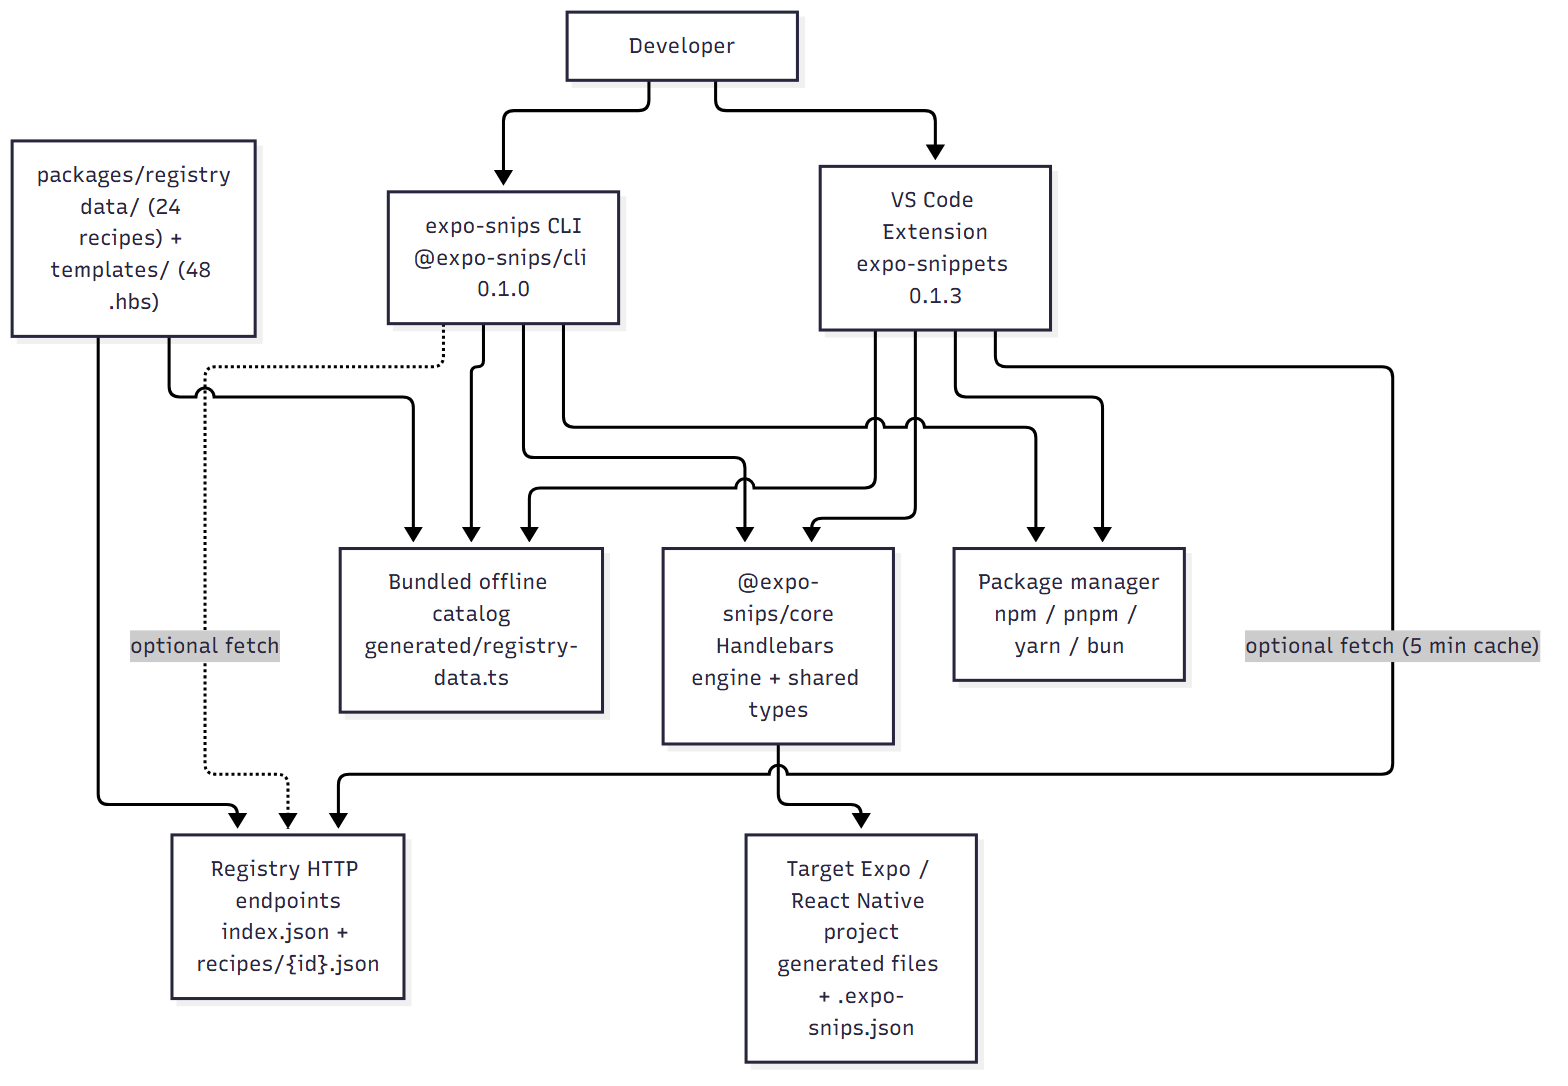
\includegraphics[width=\textwidth]{diagrams/system-architecture.png}
\caption{System architecture: clients, shared engine, catalog sources and target project}
\label{fig:system-architecture}
\end{figure}

\begin{longtable}{p{3.6cm}p{10.4cm}}
\caption{System elements}\\
\toprule
\textbf{Element} & \textbf{Responsibility and evidence} \\
\midrule

CLI client & Command parsing, interactive prompts, stack detection, orchestration and
terminal reporting. \texttt{packages/cli/src}. \\
Extension client & Command palette, completion trigger, status bar, workspace
detection, orchestration in an editor context. \texttt{packages/vscode-extension/src}. \\
Generation engine & Condition filtering and Handlebars rendering; pure functions with
no I/O. \texttt{packages/core/src}. \\
Offline catalog & Recipe arrays inlined into each client at build time
(\texttt{src/generated/registry-data.ts}, git-ignored, produced by
\texttt{scripts/prepare-registry.mjs}). \\
Registry service & Static JSON published over HTTP: \texttt{index.json} plus
per-recipe documents. \texttt{registry/}; default base
\texttt{https://registry.expo-snips.dev}. \\
Catalyst / build pipeline & Recipe source data and templates compiled into the
registry folder and into the embedded bundles.
\texttt{scripts/build-registry.mjs}, \texttt{scripts/lib/build-recipes.mjs}. \\
Target project & The user's Expo / React Native application, which receives
generated files and the \texttt{.expo-snips.json} manifest. \\
Package manager & External process used to install recipe dependencies. \\
\bottomrule
\end{longtable}

\section{Deployment topology}

\begin{itemize}
  \item \textbf{Clients} execute on the developer's machine
        (Windows, macOS or Linux).
  \item \textbf{Registry} is static hosting. The repository's own workflow deploys
        it to GitHub Pages under a \texttt{registry/} path; the code also supports
        any base URL, including a local server started with
        \texttt{pnpm serve} (default \texttt{http://localhost:3000}).
  \item \textbf{Packages} are distributed through the public npm registry.
  \item \textbf{No runtime service, message broker, cache or database exists in the
        deployed system.}
\end{itemize}

\section{Communication paths}

\begin{longtable}{p{3.2cm}p{3.4cm}p{7.4cm}}
\caption{Communication paths}\\
\toprule
\textbf{From} & \textbf{To} & \textbf{Mechanism} \\
\midrule

CLI & Registry & HTTPS GET, 10\,s abort timeout, optional; falls back to embedded catalog. \\
Extension & Registry & HTTPS GET, 10\,s abort timeout, 5-minute cache and back-off, optional. \\
CLI & Package manager & Child process (\texttt{execSync}, inherited stdio). \\
CLI & create-expo-app & Child process via \texttt{npx} (\texttt{init} only). \\
Extension & Package manager & Terminal command injection (\texttt{terminal.sendText}). \\
CLI/Extension & Target project & Local filesystem writes. \\
Clients & \texttt{@expo-snips/core} & In-process function calls (TypeScript module import). \\
Build pipeline & Registry & Local filesystem writes during CI. \\
\bottomrule
\end{longtable}

\begin{figure}[H]
\centering
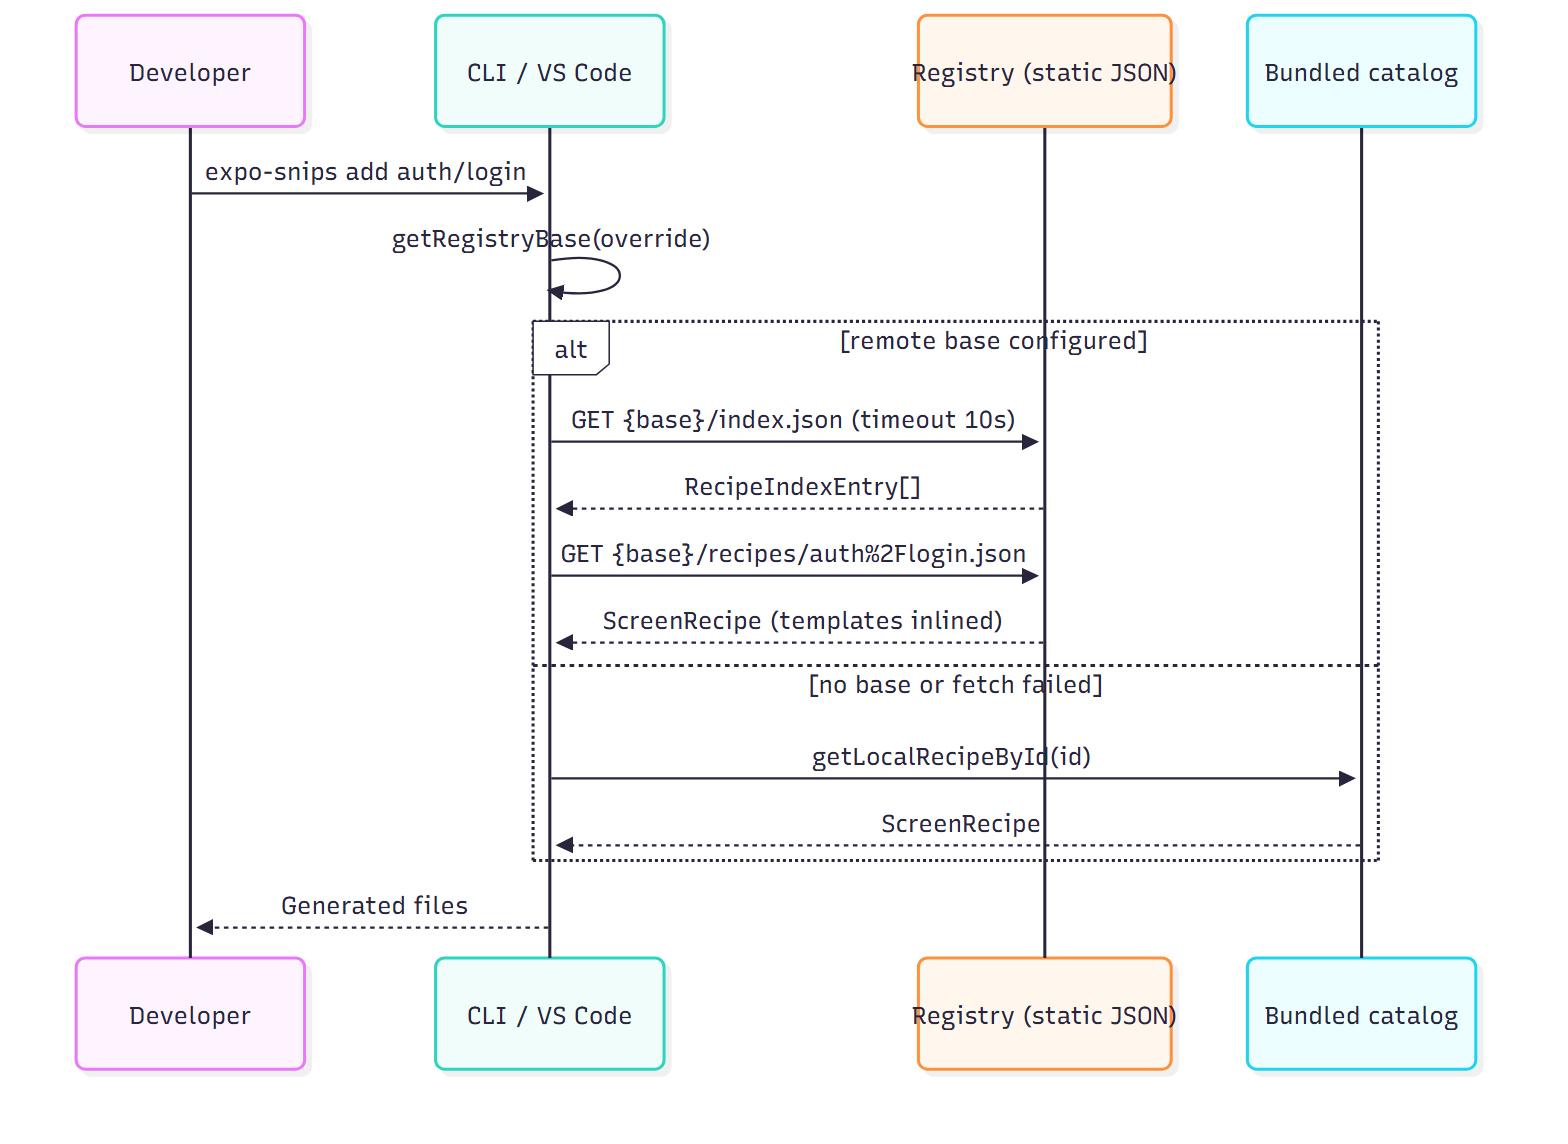
\includegraphics[width=0.92\textwidth]{diagrams/registry-api-sequence.png}
\caption{Registry resolution sequence with bundled-catalog fallback}
\label{fig:registry-api-sequence}
\end{figure}

\section{Architectural characteristics}

\begin{longtable}{p{4cm}p{10cm}}
\caption{Architectural characteristics}\\
\toprule
\textbf{Characteristic} & \textbf{Assessment} \\
\midrule

Distribution style & Local-first, offline-capable. \\
State & Stateless process; persistence only in the user's project manifest. \\
Coupling & Low-to-moderate: clients depend on the engine and on the recipe schema;
the engine has no dependency on either client. \\
Cohesion & High within each package; the recipe format is the stable contract. \\
Scalability & The catalog scales by adding files; there is no runtime scaling concern
because there is no server. \\
Failure isolation & Catalog fetch failure is contained; a failed install aborts the
CLI command after files have been written. \\
Trust boundary & The registry is trusted without verification --- the principal
architectural risk (see Chapter~\ref{ch:security}). \\
\bottomrule
\end{longtable}

\section{Key architectural decisions}

\begin{longtable}{p{1.3cm}p{5.4cm}p{7.3cm}}
\caption{Architectural decisions and rationale}\\
\toprule
\textbf{ID} & \textbf{Decision} & \textbf{Rationale / consequence} \\
\midrule

AD-01 & Inline templates into recipe JSON at build time & Consumers never need
filesystem access to templates; enables both HTTP delivery and embedded bundles.
Evidenced by \texttt{build-recipes.mjs} and the emitted recipe files. \\
AD-02 & Share one engine across clients & Guarantees identical output from CLI and
editor. Both import \texttt{getFilesForRecipe}. \\
AD-03 & Bundle the catalog in clients as well as hosting it & Guarantees offline
operation; remote registry becomes an enhancement rather than a dependency. \\
AD-04 & Recipes are data, not code & New screens need no engine change; validated by
schema. Trade-off: template strings are embedded in JSON, which is awkward to edit
and diff but trivially portable. \\
AD-05 & Use Handlebars rather than a stronger typed generator & Minimal dependency
footprint in the engine (one runtime dependency) at the cost of limited type safety
inside templates (INFERRED). \\
AD-06 & Force \texttt{nativewind} + \texttt{lucide} when \texttt{ui=shadcn} & The
shadcn-style primitives depend on NativeWind utility classes and lucide icons;
enforced rather than validated. \\
AD-07 & Persist installs in a project-local manifest & Enables update and status
workflows without any server-side account. \\
\bottomrule
\end{longtable}

\section{Constraints and limitations of the architecture}

\begin{itemize}
  \item No plugin or extension mechanism exists inside the clients; adding a screen
        means adding catalogue data, not extending the CLI.
  \item The engine's generated output depends on the recipe's \texttt{when}
        conditions being written correctly; there is no schema check that every
        supported option combination yields at least one file for every required
        path.
  \item Because templates are inlined into JSON, template content is escaped and
        difficult to review in the built registry (see the \texttt{auth/login}
        built recipe, where multi-line templates appear as single escaped lines).
  \item The extension duplicates the CLI's detection and primitive-resolution logic
        rather than importing it, so the two can drift.
\end{itemize}

\textbf{Status:} IMPLEMENTED (the first, second and fourth items are directly
observable); INFERRED (the third).
